% !TeX spellcheck = en_GB
%%%%%%%%%%%%%%%%%%%%%%%%%%%%%%%%%%%%%%%%%
% Masters/Doctoral Thesis 
% LaTeX Template
% Version 2.5 (27/8/17)
%
% This template was downloaded from:
% http://www.LaTeXTemplates.com
%
% Version 2.x major modifications by:
% Vel (vel@latextemplates.com)
%
% This template is based on a template by:
% Steve Gunn (http://users.ecs.soton.ac.uk/srg/softwaretools/document/templates/)
% Sunil Patel (http://www.sunilpatel.co.uk/thesis-template/)
%
% Template license:
% CC BY-NC-SA 3.0 (http://creativecommons.org/licenses/by-nc-sa/3.0/)
%
%%%%%%%%%%%%%%%%%%%%%%%%%%%%%%%%%%%%%%%%%

%----------------------------------------------------------------------------------------
%	PACKAGES AND OTHER DOCUMENT CONFIGURATIONS
%----------------------------------------------------------------------------------------

\documentclass[
11pt, % The default document font size, options: 10pt, 11pt, 12pt
oneside, %TODO: % Two side (alternating margins) for binding by default, uncomment to switch to one side
english, % ngerman for German
singlespacing, % Single line spacing, alternatives: onehalfspacing or doublespacing
%draft, % Uncomment to enable draft mode (no pictures, no links, overfull hboxes indicated)
%nolistspacing, % If the document is onehalfspacing or doublespacing, uncomment this to set spacing in lists to single
liststotoc, % Uncomment to add the list of figures/tables/etc to the table of contents
toctotoc, % Uncomment to add the main table of contents to the table of contents
%parskip, % Uncomment to add space between paragraphs
%nohyperref, % Uncomment to not load the hyperref package
headsepline, % Uncomment to get a line under the header
%chapterinoneline, % Uncomment to place the chapter title next to the number on one line
consistentlayout, % Uncomment to change the layout of the declaration, abstract and acknowledgements pages to match the default layout
]{./latex_template} % The class file specifying the document structure

%\usepackage[utf8]{inputenc} % Required for inputting international characters
\usepackage[T1]{fontenc} % Output font encoding for international characters
\usepackage{mathpazo} % Use the Palatino font by default
\usepackage{tabu}
\usepackage{diagbox}
\usepackage{rotating}
\usepackage{makecell}
\usepackage{float}
\usepackage{url}
\usepackage{pdfpages}
\usepackage[normalem]{ulem}
\usepackage[autostyle=true]{csquotes} % Required to generate language-dependent quotes in the bibliography

\newcommand*{\fullref}[1]{\hyperref[{#1}]{\ref*{#1} \nameref*{#1}}} % One single link

%----------------------------------------------------------------------------------------
%	MARGIN SETTINGS
%----------------------------------------------------------------------------------------

\geometry{
	paper=a4paper, % Change to letterpaper for US letter
	inner=2.5cm, % Inner margin
	outer=3.8cm, % Outer margin
	bindingoffset=.5cm, % Binding offset
	top=1.5cm, % Top margin
	bottom=1.5cm, % Bottom margin
	%showframe, % Uncomment to show how the type block is set on the page
}
\global\tabulinesep=1.2mm

%----------------------------------------------------------------------------------------
%	Glossary SETTINGS
%----------------------------------------------------------------------------------------
\usepackage{hyperref}
\usepackage[toc,nopostdot, nonumberlist]{glossaries}%acronym
\setglossarystyle{altlist}
\usepackage{xparse}
\DeclareDocumentCommand{\newdualentry}{ O{} O{} m m m m } {
	\newglossaryentry{gls-#3}{
		name={#4 : #5},
		text={#5\glsadd{#3}},
		description={#6},
		#1
	}
	\makeglossaries
	\newacronym[see={[Siehe:]{gls-#3}},#2]{#3}{#4}{#5\glsadd{gls-#3}}
}
\renewcommand{\glstextformat}[1]{\textit{#1}}
\makeglossaries

\DeclareTextFontCommand{\emph}{\bfseries\em}

%----------------------------------------------------------------------------------------
%	THESIS INFORMATION
%----------------------------------------------------------------------------------------

\thesistitle{XMPP-Grid Broker} %is used in the title and abstract, print it elsewhere with \ttitle
\supervisor{Prof.~Dr.~Andreas~\textsc{Steffen}} %is used in the title page, print it elsewhere with \supname
\examiner{} %print it elsewhere with \examname
\author{Fabian~\textsc{Hauser} and Raphael~\textsc{Zimmermann}} %is used in the title page and abstract, print it elsewhere with \authorname

\keywords{XMPP Grid Broker} % is not currently used anywhere in the template, print it elsewhere with \keywordnames
\university{\href{https://www.hsr.ch}{University of Applied Sciences Rapperswil}} %is used in the title page and abstract, print it elsewhere with \univname
\department{Department of Computer Science} %is used in the title page and abstract, print it elsewhere with \deptname

\AtBeginDocument{
\hypersetup{pdftitle=\ttitle} % Set the PDF's title to your title
\hypersetup{pdfauthor=\authorname} % Set the PDF's author to your name
\hypersetup{pdfkeywords=\keywordnames} % Set the PDF's keywords to your keywords
}

\loadglsentries{glossar}

\begin{document}

\frontmatter % Use roman page numbering style (i, ii, iii, iv...) for the pre-content pages
\pagestyle{plain} % Default to the plain heading style until the thesis style is called for the body content

%----------------------------------------------------------------------------------------
%	TITLE PAGE
%----------------------------------------------------------------------------------------

\begin{titlepage}
\begin{center}

\vspace*{.06\textheight}
{\scshape\LARGE \univname\par} % University name

{\scshape\large Department of Computer Science\par}\vspace{1.2cm} % University name
\textsc{\Large Bachelor Thesis}\\[0.5cm] % Thesis type

\HRule \\[0.4cm] % Horizontal line
{\huge \bfseries \ttitle\par}\vspace{0.4cm} % Thesis title
\HRule \\[1.5cm] % Horizontal line
 
\begin{minipage}[t]{0.4\textwidth}
\begin{flushleft} \large
\emph{Authors:}\\
\authorname % Author name - remove the \href bracket to remove the link
\end{flushleft}
\end{minipage}
\begin{minipage}[t]{0.4\textwidth}
\begin{flushright} \large
\emph{Advisor:} \\
\supname \\[1cm]
\emph{External Co-Examiner:} \\
\examname \\[1cm]
\emph{Internal Co-Examiner:} \\
\textit{not yet defined} \\[1cm]
\end{flushright}
\end{minipage}\\[3cm]
 
\vfill

{\large Spring Term 2018}\\[4cm] % Date

\includegraphics{resources/logo_hsr} % University/department logo - uncomment to place it
 
\vfill
\end{center}
\end{titlepage}
%----------------------------------------------------------------------------------------
%	License / information PAGE
%------------------------------------------

\vspace*{\fill}

\noindent \textcopyright  Copyright 2018 by Fabian Hauser and Raphael Zimmermann\\

\noindent This documentation is available under the GNU FDL License. \\

\noindent The XMPP-Grid Broker software is licensed under the AGPL-License. This does not apply to third-party libraries.

\pagebreak

%----------------------------------------------------------------------------------------
%	QUOTATION PAGE
%----------------------------------------------------------------------------------------

\vspace*{0.1\textheight}

{\noindent\huge\textit{DON`T PANIC}\par\vspace{10pt}}

\noindent\enquote{\itshape It looked insanely complicated, and this was one of the reasons why the snug plastic cover it fitted into had the words DON`T PANIC printed on it in large friendly letters.}\bigbreak

\hfill The Hitchhiker`s Guide to the Galaxy

%----------------------------------------------------------------------------------------
%	ABSTRACT PAGE
%----------------------------------------------------------------------------------------

\begin{abstract}
\addchaptertocentry{\abstractname} % Add the abstract to the table of contents
\end{abstract}

%----------------------------------------------------------------------------------------
%	MANAGEMENT SUMMARY
%----------------------------------------------------------------------------------------

\chapter{Management Summary}
\addchaptertocentry{\abstractname} % Add the abstract to the table of contents
%The Thesis Management Summary is written here (and usually kept to just this page).
% Das Management Summary richtet sich in der Praxis an die "Chefs des Chefs",
%  d.h. an die Vorgesetzten des Auftraggebers (diese sind in der Regel keine Fachspezialisten).
%  Die Sprache soll knapp, klar und stark untergliedert sein. Zu verwenden ist folgenden Gliederung:
% - Ausgangslage
% - Vorgehen, Technologien
% - Ergebnisse
% - Ausblick (optional)

% prototype demonstrates feasability
% further conceptual refinement needed
% implemenetation is complex - but doable.

%----------------------------------------------------------------------------------------
%	ACKNOWLEDGEMENTS
%----------------------------------------------------------------------------------------

\begin{acknowledgements}
\addchaptertocentry{\acknowledgementname} % Add the acknowledgements to the table of contents
We would like to thank our advisor, Prof.~Dr.~Andreas~Steffen, for his continuous support and helpful comments.

\end{acknowledgements}

%----------------------------------------------------------------------------------------
%	LIST OF CONTENTS PAGES
%----------------------------------------------------------------------------------------

\setcounter{tocdepth}{2}
\tableofcontents % Prints the main table of contents

%----------------------------------------------------------------------------------------
%	DEDICATION
%----------------------------------------------------------------------------------------

%TODO
%\dedicatory{For/Dedicated to/To my\ldots}

%----------------------------------------------------------------------------------------
%	THESIS CONTENT - CHAPTERS
%----------------------------------------------------------------------------------------

\mainmatter % Begin numeric (1,2,3...) page numbering

\pagestyle{thesis} % Return the page headers back to the "thesis" style

% !TeX spellcheck = en_GB
\newcommand{\code}{\texttt}
\chapter{Introduction}
\label{sec:introduction}

In this chapter, we introduce the terminology and background of our thesis task, to conclude in the motivation and legitimisation of our thesis.

\section{Terminology}
Taking into account that the intended audience for this thesis are developers and operators of security reporting systems, 
we mostly use the  Security Automation and Continuous Monitoring (SACM) terminology~\cite{ietf-sacm-terminology-14}
and thereby follow the same guidelines as the XMPP grid draft~\cite{ietf-mile-xmpp-grid-05}.

\section{Background}

The following sections introduce the underlying XMPP protocol and the relevant extensions (\glspl{xep}) of the XMPP grid draft as well as a summary of it and the corresponding XMPP terminology.

\subsection{XMPP (eXtensible Messaging and Presence Protocol)}
The Extensible Messaging and Presence Protocol (in short \gls{xmpp}) is an open protocol that enables the near-real-time exchange of small data between any network endpoints, hereafter called \glspl{platform}~\cite{rfc6120}.
While it was originally designed as an Instant Messaging (IM) protocol, it can be used for a wide range of data exchange applications~\cite{ieee-xplore-stream-xml-xmpp}.

XMPP is made of small building blocks defined in the core protocol~\cite{rfc6120} and numerous extensions called \glspl{xep}~\cite{xep-0001}.
The core is comprised of functionality for setup and encryption of communication channels, \gls{xml} streams, error handling and more. Additional functionality such as \gls{service-discovery}~\cite{xep-0030} and \gls{publish-subscribe}~\cite{xep-0060} are defined in separate extensions.

Although XMPP supports peer-to-peer communication, it is often used in a traditional client-server architecture.
A client (\gls{platform}) can send data to any addressable entity (any other \glspl{platform}) using \Gls{jabber} Identifiers, hereafter called \gls{jid}. If the \gls{jid} of the receiver has a different domainpart than the current server (\gls{controller}), the message is forwarded to the responsible XMPP server under its domain~\cite{rfc6120}.

The data exchanged over XMPP is \gls{xml} which makes the protocol structured and extensible, but leads to some protocol overhead.
XMPP communicates over unidirectional data streams with a server, which are basically long-lived \gls{tcp} connections.
The client opens a channel to the server over this connection, and the server opens one back (i.e. \code{<stream>} XML tags). In both streams, an XML document is opened after the connection is established.
During the conversation, an arbitrary amount of \glspl{stanza} (specified XML child elements) are written to the stream.
Before a connection may be terminated, the root element is closed (i.e. \code{</stream>}) and both streams form valid XML documents~\cite{rfc6120}\cite{professional-xmpp}.

The core \gls{stanza} types are \glspl{message}~(\code{<message/>}), \gls{presence}~(\code{<presence/>}) and\\
\gls{info-query}~(\code{<iq/>}).
\Glspl{message} can contain arbitrary data similar to email but are optimised for immediate delivery.
\Gls{presence} \glspl{stanza} deal with network availability and the propagation of user presence information.
An \gls{info-query} \gls{stanza} consists of a request and response (similar to the GET and POST HTTP methods), which is used for feature negotiation, configuration and general information exchange.
Because of these coarse semantics, XMPP provides a generalized communication layer~\cite{rfc6120}\cite{ieee-xplore-stream-xml-xmpp}.

Figure~\ref{fig:xmpp-overview} illustrates an example setup with two servers and three clients.

\begin{figure}[h]
	\centering
	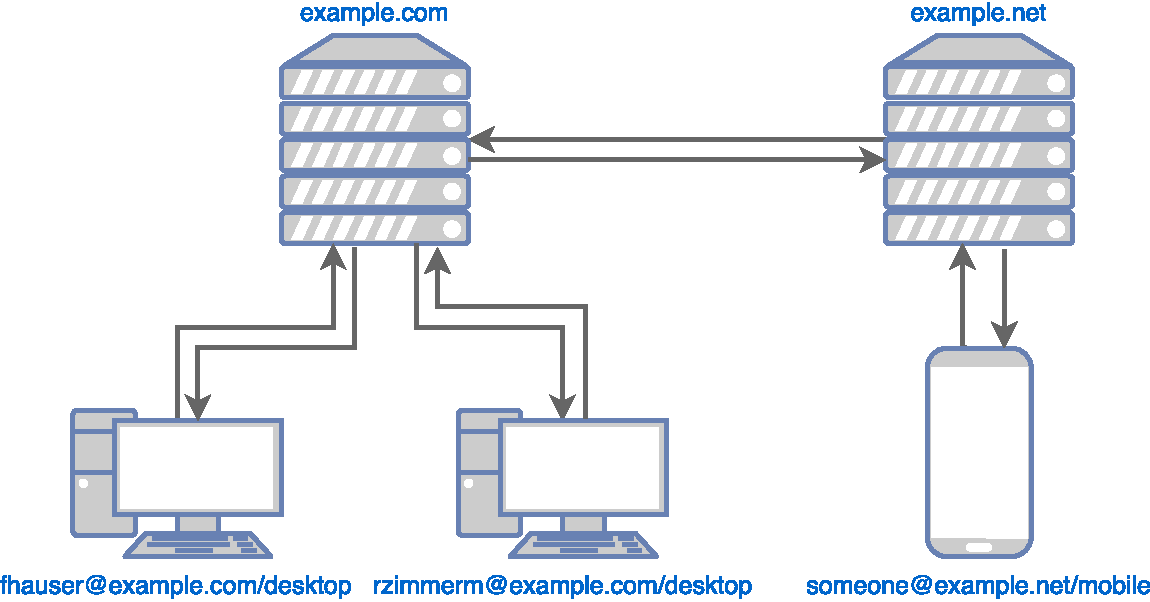
\includegraphics[width=0.8\linewidth]{resources/xmpp_overview.pdf}
	\caption{Two XMPP domains (servers), one with two users and one with one mobile user.}
	\label{fig:xmpp-overview}
\end{figure}

\subsection{Relevant XMPP Extensions}

The XMPP grid draft~\cite{ietf-mile-xmpp-grid-05} is based on multiple \glspl{xep}, most notably \gls{publish-subscribe}. In this section, we give an overview of the most relevant used \glspl{xep}.

\paragraph{XEP-0004: \gls{data-forms}} is a flexible protocol that can be used in workflows such as service configuration as well as for application-specific data description and reporting. The protocol provides form processing, common field types and extensibility mechanisms~\cite{xep-0004}.

\paragraph{XEP-0030: \gls{service-discovery}} enables entities to discover information about the identity and capabilities of other entities, e.g. whether the entity is a server or not, or items associated with an entity, e.g. a list of \gls{publish-subscribe} nodes~\cite{xep-0030}.

\paragraph{XEP-0059: \Gls{result-set-management}} allows entities to manage the receipt of large result sets, e.g. by paging through the result or limiting the number of results. \gls{result-set-management} is often desired when dealing with large dynamic result sets, as from service discovery or publish-subscribe, and time or other resources are limited~\cite{xep-0059}.

\subsubsection{XEP-0060: \Gls{publish-subscribe}}
The \gls{publish-subscribe} Extension, hereafter referred to as \gls{pubsub} or \gls{broker}, enables XMPP entities (\gls{provider}) to broadcast information via \glspl{topic} to subscribed entities (\gls{consumer})~\cite{xep-0060}.

Nodes, hereafter referred to as \glspl{topic}, are the communication hubs. Entities can create topics and configure them, e.g. set up subscription timeouts, limit publish and subscription rights. The configuration mechanism is based on data forms (XEP\babelhyphen{nobreak}0004).

The protocol defines a hierarchy of six affiliations of which only the implementation of `owner` and `none` is required. The implementation of the remaining four affiliations is recommended. An owner of a topic can manage the subscriptions and affiliations of other entities associated with a given topic.

To make the creation of topics simpler for clients, \gls{pubsub} defines five topic access models ("node access models"): open, presence, roaster, authorize and whitelist.

The open model allows uncontrolled access while presence and roaster are specific for IM. Using the authorize model, the owner has to approve all subscription requests. The whitelist model enables the owner to maintain a list of entities that are allowed to subscribe.

\subsection{IETF Internet-Draft: Using XMPP for Security Information Exchange}\label{sec:ietf-internet-draft-using-xmpp-for-security-information-exchange}
This IETF Internet draft describes how the XMPP protocol enhanced with the previously discussed XEPs, most notably the \gls{pubsub} extension, can be used for the exchange and distribution of security-relevant information between network devices.

One of the primary motivation for using XMPP for this task is the fast propagation of such security-relevant data.
Using XMPP for such a task also comes with its downsides. Most notably, because the XMPP server (\gls{broker}/\gls{controller}) is the central configuration component in charge of managing access permission, its compromisation has serious consequences.

The draft describes a trust model, thread model as well as specific countermeasures, e.g. to use at least TLS 1.2. These countermeasures also define restrictions of the XMPP protocol and its extensions, e.g. by limiting the topic access models of \gls{pubsub} to whitelist and authorized only~\cite{ietf-mile-xmpp-grid-05}.

\section{Motivation}
In this section, we legitimate this thesis and explain the value and applicability of our proposed solution.

\subsection{Present situation}
The IETF standard draft \emph{Using \gls{xmpp} for Security Information Exchange} \cite{ietf-mile-xmpp-grid-05} as summarised in section \ref{sec:ietf-internet-draft-using-xmpp-for-security-information-exchange} defines a protocol to exchange security-relevant information between endpoints.
The draft was created by the Managed Incident Lightweight Exchange (MILE) Working Group to support computer and network security incident management.

To demonstrate the viability of the draft a rapid prototype was developed in November~2017~\cite{xmpp-grid-prototype}.

\subsection{Problem and Solution}
Currently, there exists no implementation of the \gls{xmpp} grid draft management functionality which is ready for production use regarding usability and security.

To solve this problem, a graphical interface with bindings to a suitable \gls{broker} must be proposed and implemented.
The interface should permit network administrators to manage and review \glspl{topic}, persisted items and \glspl{platform}. Additionally, access and publishing permissions of \glspl{topic} and \glspl{platform} must be manageable.

\subsubsection*{} %This is needed, so that not the next page is referenced.
\label{lastpage} %TODO: This label should be positioned below above the last paragraph

\cleardoublepage
%----------------------------------------------------------------------------------------
%	BIBLIOGRAPHY
%----------------------------------------------------------------------------------------
\backmatter
\pagenumbering{Roman}

\bibliographystyle{abbrv}
\bibliography{references}
\addcontentsline{toc}{chapter}{Bibliography}


%----------------------------------------------------------------------------------------
%	LIST OF FIGURES/TABLES PAGES
%----------------------------------------------------------------------------------------

\listoffigures % Prints the list of figures

\listoftables % Prints the list of tables

%----------------------------------------------------------------------------------------
%	GLOSSARY
%----------------------------------------------------------------------------------------

\glsaddall
\printglossary


%----------------------------------------------------------------------------------------
%	THESIS CONTENT - APPENDICES
%----------------------------------------------------------------------------------------


\appendix % Cue to tell LaTeX that the following "chapters" are Appendices
\chapter{Appendices}
\setcounter{secnumdepth}{3}
\renewcommand{\thechapter}{A}
\section{Task Description}\label{sec:task-description}

\includepdf[pages=-,scale=.9,frame]{../task-description-signed.pdf}
\section{Project Plan}\label{sec:project-plan}
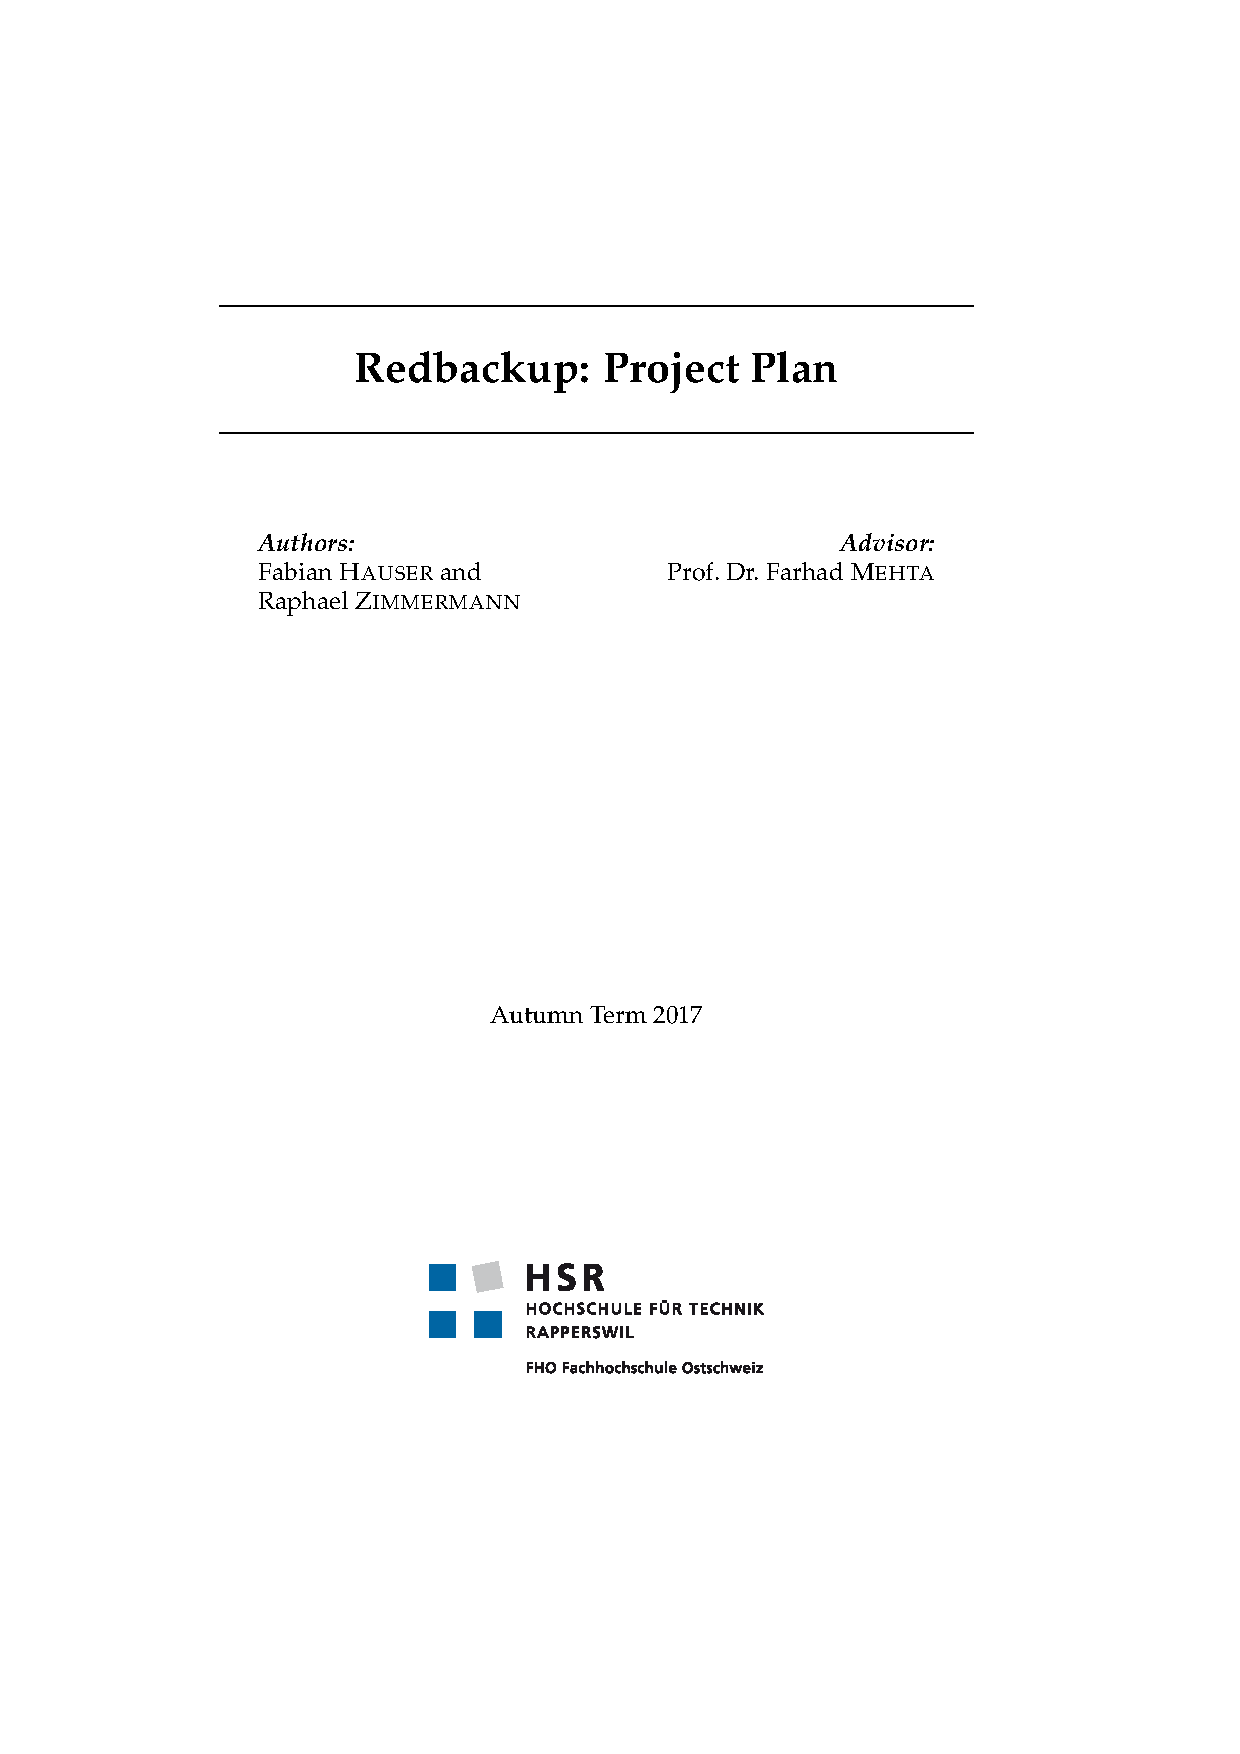
\includepdf[pages=-,scale=.9,frame]{../project-plan/project-plan.pdf}
\section{Development Guide}\label{sec:development-guide}
\includepdf[pages=-,scale=.9,frame]{../development-guide.pdf}
\section{Time Accounting}\label{sec:time-accounting}

\includepdf[pages=-,scale=.9,frame]{../time-accounting.pdf}
\section{Meeting Minutes}\label{sec:meeting-minutes}
\includepdf[pages=-,scale=.9,frame]{../meeting-minutes/meeting-minutes.pdf}


%----------------------------------------------------------------------------------------
%	DECLARATION PAGE
%----------------------------------------------------------------------------------------

\begin{declaration}
\addchaptertocentry{\authorshipname} % Add the declaration to the table of contents
\noindent We, \authorname, declare that this thesis and the work presented in it are our own, original work.  All the sources we consulted and cited are clearly attributed. We have acknowledged all main sources of help. \\

\noindent Fabian Hauser\\[2em]
\rule[0.5em]{25em}{0.5pt}\\ % This prints a line for the signature
\noindent Raphael Zimmermann\\[2em]
\rule[0.5em]{25em}{0.5pt}\\ % This prints a line for the signature 
\noindent Rapperswil, \today
\end{declaration}

\cleardoublepage


%----------------------------------------------------------------------------------------

\end{document}  
